\documentclass[xcolor=table,dvipsnames,table]{beamer}
\mode<presentation>
\usetheme{boxes}
\setbeamertemplate{navigation symbols}{}
% http://www.latex-community.org/forum/viewtopic.php?f=4&t=6694
\setbeamertemplate{navigation symbols}{\raisebox{5pt}{\makebox[\paperwidth]{\hfill\makebox[10pt]{\scriptsize\insertframenumber\vspace{1ex}}}}}
%\setbeamertemplate{footline}[frame number]
\setbeamertemplate{blocks}[shadow=false]
%\setbeamercolor*{block title}{fg=structure,bg=RoyalBlue!10}
\setbeamercolor*{block title example}{fg=structure,bg=RoyalBlue!10}
%\setbeamercolor*{block title example}{fg=BrickRed,bg=Goldenrod!10}
\setbeamercolor*{block title alerted}{fg=white,bg=black}
\addtobeamertemplate{block begin}{\pgfsetfillopacity{0.8}}{\pgfsetfillopacity{1}}
%\rowcolors{0}{RoyalBlue!20}{RoyalBlue!5}
\setbeamertemplate{caption}{\raggedright\insertcaption\par}

%\DeclareGraphicsRule{*}{mps}{*}{}

\usepackage{latexsym}
\usepackage{hyperref}
\usepackage{tikz}
\usetikzlibrary{calc,shapes,arrows,shadows,shapes.callouts,shapes.arrows,chains,positioning,trees}
\usepackage{solution}
\usepackage{calc}
\usepackage{pifont}
\usepackage{algorithmic}
\usepackage{pdfcomment}
\usepackage{color}

\newcommand{\cmark}{\ding{51}}
\newcommand{\xmark}{\ding{55}}

\newcommand{\highlight}[1]{{\color{blue}{#1}}}
\newcommand{\mycite}[1]{{\color{darkgray}{\footnotesize [#1]}}}

\DeclareMathOperator*{\argmin}{arg\,min}
\DeclareMathOperator*{\argmax}{arg\,max}
\DeclareMathOperator{\sign}{sign}
\DeclareMathOperator{\cnt}{Count}

\newcounter{mycallout}

\newcommand{\callouts}[3]{%
  \stepcounter{mycallout}
  \tikz[remember picture,baseline]{\node[anchor=base,inner sep=0,outer sep=0]%
    (\themycallout) {\colorbox{#1!20}{#3}};\pause\node[overlay,rectangle callout,%
    callout relative pointer={(0cm,0.5cm)},fill=#1!20] at ($(\themycallout.south)+(-0cm,-0.7cm)$){#2};}%
    }%

\raggedright

\newcount\lecturecount
\lecturecount=0
\AtBeginLecture{%
    \advance\lecturecount by 1
    \date{}
    \begin{frame}
    \begin{center}
    \titlepage
    \ifnum\lecturecount=1
    Part \the\lecturecount: \insertlecture
    \else
    Part \the\lecturecount: \insertlecture
    \fi
    \end{center}
    \end{frame}
}

\addtobeamertemplate{block begin}{\setlength\abovedisplayskip{0pt}}

%\newcommand{\example}[1]{{\color{BrickRed!50}{#1}}}
\newcommand{\maths}[1]{{\color{RoyalBlue!50}{#1}}}
\newcommand{\reference}[1]{{\color{RoyalBlue!30}\tiny [from #1]}}
\newcommand{\koehnref}{\reference{\href{http://www.statmt.org/book}{P.Koehn SMT book slides}}}


\begin{document}

\title{\color{MidnightBlue}Natural Language Processing}

\author{Anoop Sarkar \\ {\color{RoyalBlue!70}{\href{http://anoopsarkar.github.io/nlp-class}{anoopsarkar.github.io/nlp-class}}}}
\institute{\color{BrickRed}Simon Fraser University}
%\date{}
     
{
\addtocounter{framenumber}{-1}
\begin{frame}
\begin{center}
\vspace{8mm}

\includegraphics[scale=0.35]{figures/natlang-cky-logo}
\end{center}
\titlepage
\end{frame}
}



%\author{}
%\institute{}

\lecture{Classification tasks in NLP}{}

\section{Classification tasks in NLP}
\frame{\tableofcontents[currentsection]}

\begin{frame}
\frametitle{Sentiment classification: Movie reviews}
\begin{itemize}
\item {\color{red} neg} unbelievably disappointing 
\item {\color{green} pos} Full of zany characters and richly applied satire, and some great plot twists
\item {\color{green} pos} this is the greatest screwball comedy ever filmed  
\item {\color{red} neg} It was pathetic. The worst part about it was the boxing scenes.
\end{itemize}
\end{frame}

\begin{frame}
\frametitle{Intent Detection}
\begin{itemize}
\item {\color{blue} ADDR\_CHANGE} I just moved and want to change my address. 
\item {\color{blue} ADDR\_CHANGE} Please help me update my address.  
\item {\color{blue} FILE\_CLAIM} I just got into a terrible accident and I want to file a claim. 
\item {\color{blue} CLOSE\_ACCOUNT} I'm moving and I want to disconnect my service.
\end{itemize}
\end{frame}

\begin{frame}
\frametitle{Prepositional Phrases}
\begin{itemize}[<+->]
\item noun attach: {\em I bought \textbf{the shirt with pockets}}
\item verb attach: {\em I \textbf{bought} the shirt \textbf{with my credit card}}
\item noun attach: {\em I washed \textbf{the shirt with mud}}
\item verb attach: {\em I \textbf{washed} the shirt \textbf{with soap}}
\item Attachment depends on the meaning of the entire sentence -- needs world knowledge, etc.
\item Maybe there is a simpler solution: we can attempt to solve it using heuristics or associations between words
\end{itemize}
\end{frame}

\begin{frame}
\frametitle{Ambiguity Resolution: Prepositional Phrases in English}
  \begin{itemize}[<+->]
  \item Learning Prepositional Phrase Attachment: Annotated Data
\begin{tabular}{|cccc|c|}
\hline
$v$    &     $n_1$   &      $p$ & $n_2$ &       Attachment\\
\hline
join   &   board    &   as &  director & V \\
is       & chairman  &  of  & N.V.    & N \\
using  &   crocidolite & in  & filters & V \\
bring  &   attention  & to  & problem &  V \\ 
is      &  asbestos   & in &  products & N \\
making &   paper    &   for & filters & N \\
including & three     &  with & cancer &  N \\
$\vdots$ & $\vdots$ & $\vdots$ & $\vdots$ & $\vdots$ \\
\hline
\end{tabular}
  \end{itemize}

\end{frame}

\begin{frame}
\frametitle{Prepositional Phrase Attachment}
\begin{tabular}{|l|c|}  \hline
Method & Accuracy \\ \hline
Always noun attachment & 59.0 \\
Most likely for each preposition & 72.2 \\
Average Human (4 head words only) & 88.2 \\
Average Human (whole sentence) & 93.2 \\  \hline
\end{tabular}

\end{frame}

\begin{frame}
\frametitle{Back-off Smoothing}
\begin{itemize}[<+->]
\item Random variable $a$ represents attachment. 
\item $a = n_1$ or $a = v$ (two-class classification)
\item We want to compute probability of noun attachment: $p(a = n_1 \mid v, n_1, p, n_2)$. 
\item Probability of verb attachment is $1 - p(a = n_1 \mid v, n_1, p, n_2)$.
\end{itemize}
\end{frame}

\begin{frame}
\frametitle{Back-off Smoothing}
\begin{enumerate}
\item<1-> If $f(v,n_1,p,n_2) > 0$ and $\hat{p} \neq 0.5$
{\small
\[ \hat{p}(a_{n_1} \mid  v,n_1,p,n_2) = \frac{ f(a_{n_1},v,n_1,p,n_2) }{ f(v,n_1,p,n_2)
} \]
}
\item<2-> Else if $f(v,n_1,p) + f(v,p,n_2) + f(n_1,p,n_2) > 0$ \\
and $\hat{p} \neq 0.5$
{\small
\[ \hat{p}(a_{n_1} \mid  v,n_1,p,n_2) = \frac{ f(a_{n_1},v,n_1,p) + f(a_{n_1},v,p,n_2) +
  f(a_{n_1},n_1,p,n_2) }{ f(v,n_1,p) + f(v,p,n_2) + f(n_1,p,n_2) } \]
  }
\item<3-> Else if $f(v,p) + f(n_1,p) + f(p,n_2) > 0$
{\small
\[ \hat{p}(a_{n_1} \mid  v,n_1,p,n_2) = \frac{ f(a_{n_1},v,p) + f(a_{n_1},n_1,p) +
  f(a_{n_1},p,n_2) }{ f(v,p) + f(n_1,p) + f(p,n_2) } \]
}
\item<4-> Else if $f(p) > 0$ (try choosing attachment based on preposition alone)
{\small
\[ \hat{p}(a_{n_1} \mid  v,n_1,p,n_2) = \frac{ f(a_{n_1},p) }{ f(p) } \]
}\item<5-> Else {\small
\( \hat{p}(a_{n_1} \mid  v,n_1,p,n_2) = 1.0 \)
}
\end{enumerate}
\end{frame}

\begin{frame}
\frametitle{Prepositional Phrase Attachment: Results}
  \begin{itemize}[<+->]
  \item {\bf Results (Collins and Brooks 1995)}: 84.5\% accuracy \\
  with the use of some limited word classes for dates, numbers, etc.
  \item {\bf Toutanova, Manning, and Ng, 2004}: \\
use sophisticated smoothing model for PP attachment\\
86.18\% with words \& stems; with word classes: 87.54\%
  \item {\bf Merlo, Crocker and Berthouzoz, 1997}:\\
 test on multiple PPs, generalize disambiguation of 1 PP to 2-3 PPs\\
%14 structures possible for 3PPs assuming a single verb: all 14 are attested in the Treebank\\
%same model as CB95; but generalized to dealing with upto 3PPs\\
1PP: 84.3\% \ \ 2PP: 69.6\% \ \ 3PP: 43.6\% \\
  \end{itemize}
\end{frame}

\author{Angel Xuan Chang \\ 
  {\color{RoyalBlue!70}{\href{http://angelxuanchang.github.io/nlp-class}{angelxuanchang.github.io/nlp-class}}} \\
  {\color{gray}{adapted from lecture slides from \\ Anoop Sarkar, Danqi Chen and Karthik Narasimhan}}
}

\lecture{Probabilistic Classifiers}{}

\begin{frame}
\frametitle{Classification Task}
\begin{itemize}[<+->]
\item Input: 
  \begin{itemize}
  \item A document \highlight{$d$} 
  \item a set of classes \highlight{$C = \{c_1, c_2, \ldots, c_m\}$}
  \end{itemize}
\item Output: Predicted class \highlight{$c$} for document \highlight{$d$}
\item Example:
  \begin{itemize}
  \item {\color{red} neg} unbelievably disappointing 
  \item {\color{green} pos} this is the greatest screwball comedy ever filmed  
  \end{itemize}
\end{itemize}
\end{frame}

\begin{frame}
\frametitle{Supervised learning: Let's use statistics!}
\begin{itemize}[<+->]
\item Inputs: 
  \begin{itemize}
  \item Set of \highlight{$m$} classes \highlight{$C = \{c_1, c_2, \ldots, c_m\}$}
  \item Set of \highlight{$n$} {\em labeled} documents: \highlight{$\{(d_1, c_1), (d_2, c_2), \ldots, (d_n, c_n)\}$}
  \end{itemize}
\item Output: Trained classifier \highlight{$F: d \rightarrow c$}
  \begin{itemize}
  \item What form should \highlight{$F$} take?
  \item How to learn \highlight{$F$}?
  \end{itemize}
\end{itemize}
\note{Data-driven approach. Let machine figure out the best function to use}
\end{frame}

\begin{frame}
\frametitle{Types of supervised classifiers}
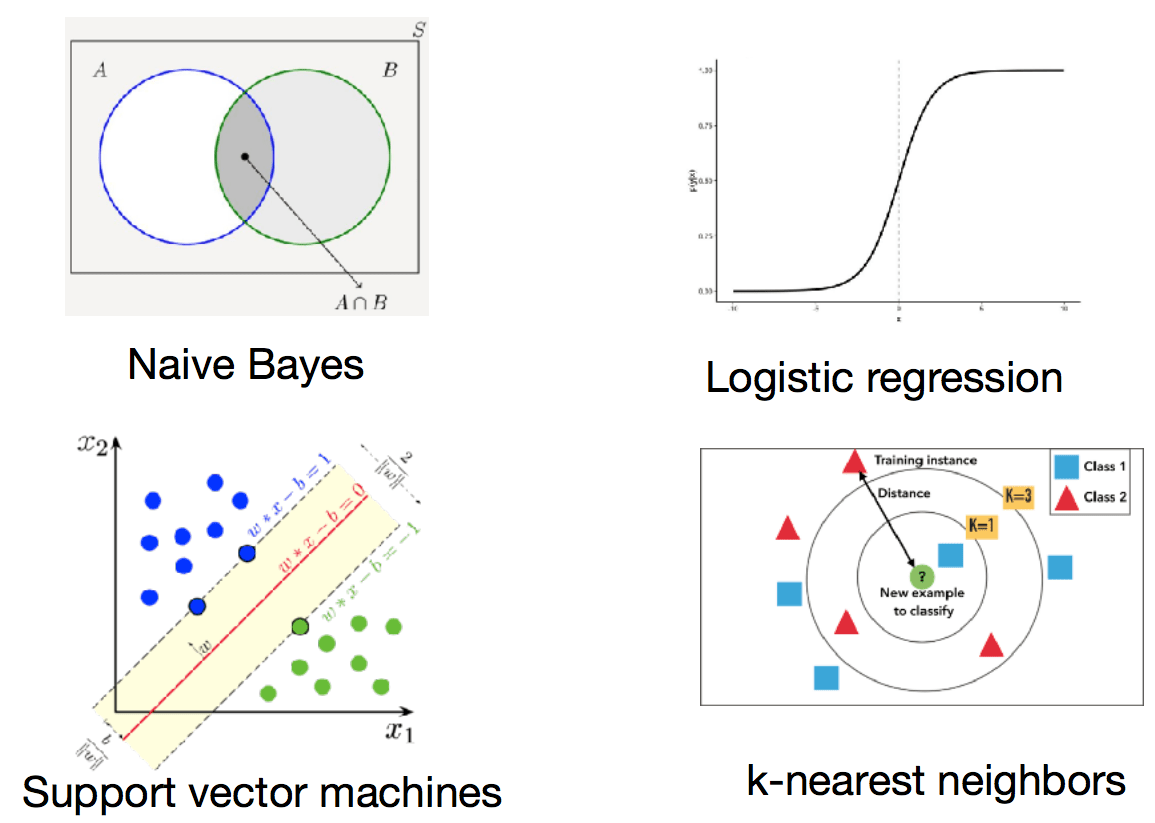
\includegraphics[scale=0.27]{figures/classifiers/supervised.png}
\end{frame}

\section{Naive Bayes Classifier}
\frame{\tableofcontents[currentsection]}

\begin{frame}
\frametitle{Naive Bayes Classifier}
\begin{itemize}[<+->]
\item \textbf{x} is the input that can be represented as $d$ independent features $f_j$, $1 \leq j \leq d$
\item $y$ is the output classification
\item $P(y \mid {\bf x}) = \frac{P(y) \cdot P({\bf x} \mid y)}{P({\bf x})}$ (Bayes Rule)
\item $P({\bf x} \mid y) = \prod_{j=1}^{d} P(f_j  \mid y)$
\item $P(y \mid {\bf x}) \propto P(y) \cdot  \prod_{j=1}^{d} P(f_j  \mid y) $
\item We can ignore $P({\bf x})$ in the above equation because it is a constant scaling factor for each $y$.
\end{itemize}
\end{frame}

\begin{frame}
\frametitle{Naive Bayes Classifier for text classification}
\begin{itemize}[<+->]
\item For text classificaiton: input $\textbf{x} = document \textbf{d} = (w_1, \ldots, w_k)$, 
\item Use as our features the words $w_j$, $1 \leq j \leq |V|$ where $V$ is our vocabulary 
\item $c$ is the output classification
\item Assume that position of each word is irrelevant and that the words are \highlight{conditionally independent} given class $c$
\begin{equation*}
P(w_1, w_2, \ldots, w_k | c) = P(w_1|c) P(w_2|c) \ldots P(w_k|c) 
\end{equation*} 
\item Maximum a posteriori estimate
\begin{equation*}
c_{\text{MAP}} = \argmax_{c} P(c) P(d|c)  = \argmax_{c} \hat{P}(c) \prod_{i=1}^{k} \hat{P}(w_i | c)
\end{equation*}
\end{itemize}
\end{frame}

\begin{frame}
\frametitle{Bag of words}
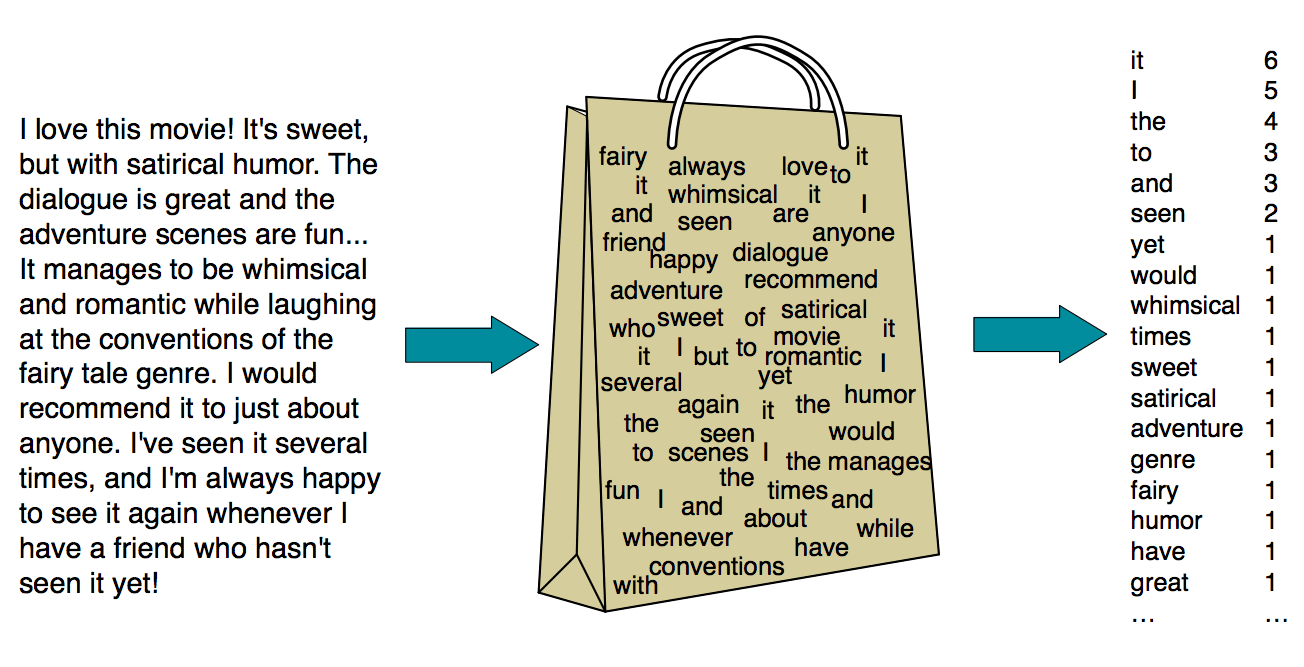
\includegraphics[scale=0.25]{figures/classifiers/bow.png}
\end{frame}

\begin{frame}
\frametitle{Estimating probabilities}
\begin{block}{Maximum likelihood estimate}
\begin{equation*}\hat{P}(c_j) = \frac{\cnt(c_j)}{n}\end{equation*} \\
\pause
\begin{equation*}\hat{P}(w_i | c_j) = \frac{\cnt(w_i, c_j)}{\sum_{w \in V}[\cnt(w, c_j)]}\end{equation*}
\end{block}
\pause
\begin{block}{Smoothing}
\begin{equation*}\hat{P}(w_i | c) = \frac{\cnt(w_i, c) + \alpha}{\sum_{w \in V}[\cnt(w, c_j) + \alpha ]}\end{equation*}
\note{simple, easy to use, effective in practice}
\end{block}
\end{frame}

\begin{frame}
\frametitle{Overall process}
Input: Set of labeled documents: $\{(d_i, c_i)\}_{i=1}^n$
\begin{itemize}[<+->]
\item Compute vocabulary $V$ of all words
\item Calculate \begin{equation*}\hat{P}(c_j) = \frac{\cnt(c_j)}{n}\end{equation*}
\item Calculate \begin{equation*}\hat{P}(w_i | c_j) = \frac{\cnt(w_i, c_j) + \alpha}{\sum_{w \in V}[\cnt(w, c_j) + \alpha ]}\end{equation*}
\item Prediction: Given document $d = (w_1, \ldots, w_k)$
\begin{equation*}
c_{\text{MAP}} = \argmax_{c} \hat{P}(c) \prod_{i=1}^{k} \hat{P}(w_i | c)
\end{equation*}
\end{itemize}
\note{n = Total number of docs}
\note{MAP = Maximum a posteriori}
\end{frame}

\begin{frame}
\frametitle{Naive Bayes Example}
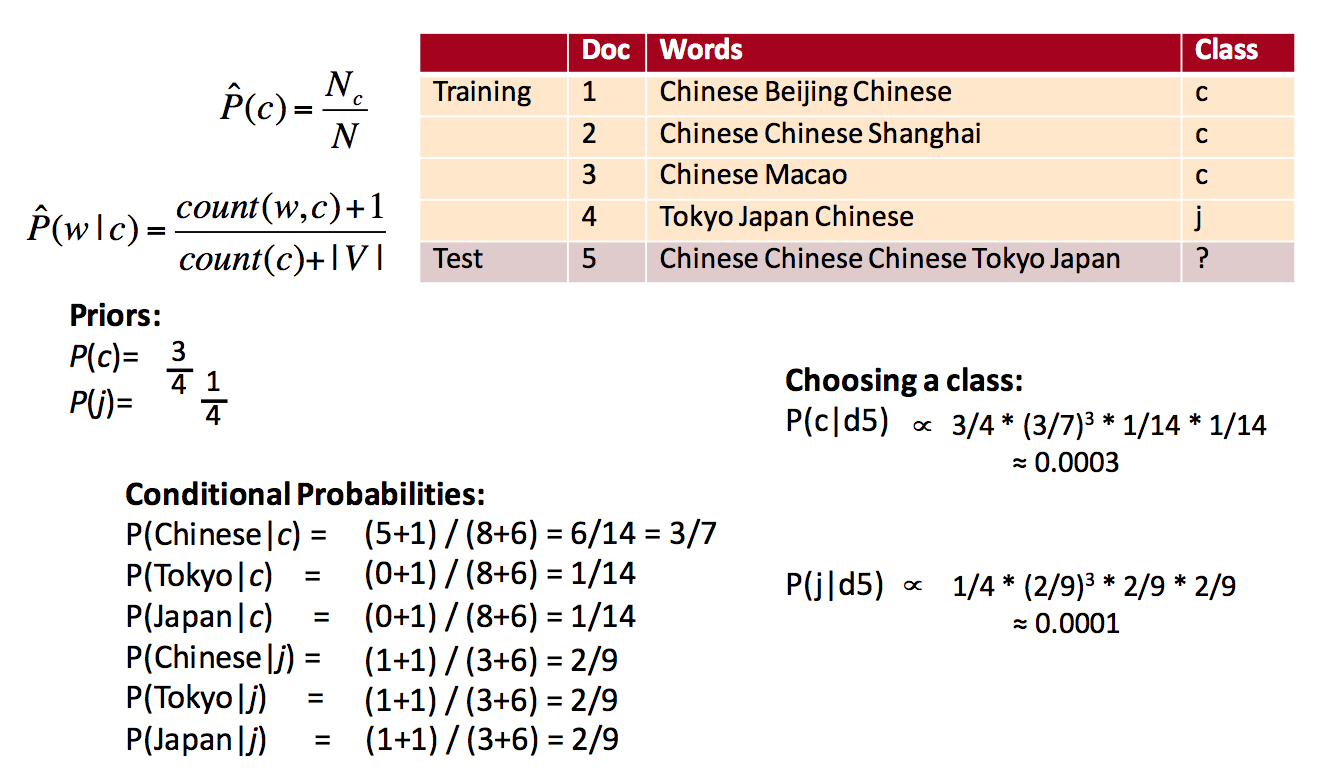
\includegraphics[scale=0.25]{figures/classifiers/nbexample.png}
\end{frame}

\begin{frame}
\frametitle{Tokenization}
\begin{block}{Tokenization matters - it can affect your vocabulary}
\begin{itemize}[<+->]
  \item {\em aren't}
    \framebox{aren't} \\
    \framebox{arent} \\
    \framebox{are} \framebox{n't} \\
    \framebox{aren} \framebox{t} \\
  \item Emails, URLs, phone numbers, dates, emoticons 
\end{itemize}
\end{block}
\end{frame}

\begin{frame}
\frametitle{Features}
\begin{itemize}[<+->]
\item Remember: Naive Bayes can use any set of features
\item Captitalization, subword features (end with -ing), etc
\item Domain knowledge crucial for performance
\end{itemize}

\pause
\begin{block}{Top features for spam detection}
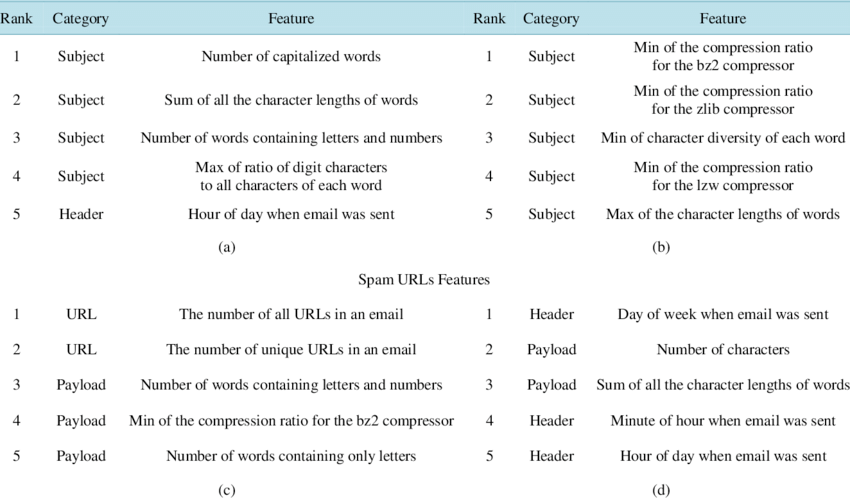
\includegraphics[scale=0.25]{figures/classifiers/features.png}
\\
\mycite{Alqatawna et al, IJCNSS 2015}
\end{block}
\end{frame}

\begin{frame}
\frametitle{Evaluation}
\begin{itemize}[<+->]
\item Table of prediction (binary classification)
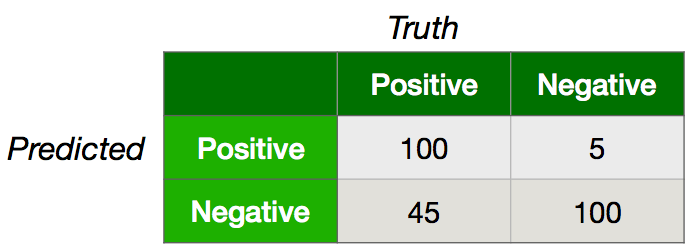
\includegraphics[scale=0.25]{figures/classifiers/evalex1.png}
\item Ideally we want to get \\
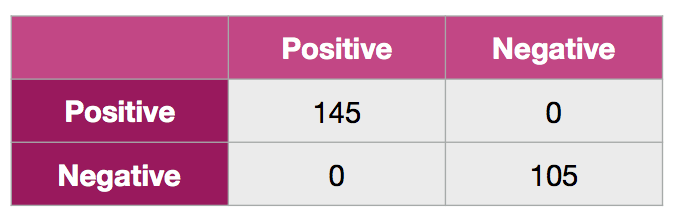
\includegraphics[scale=0.25]{figures/classifiers/evalex0.png}
\end{itemize}
\end{frame}

\begin{frame}
\frametitle{Evaluation Metrics}
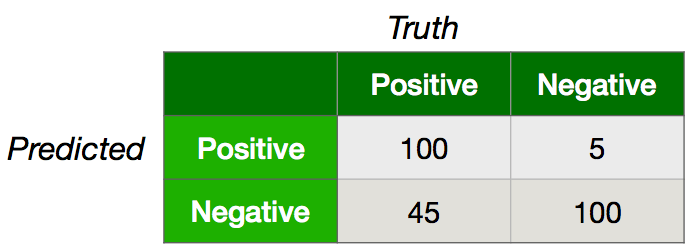
\includegraphics[scale=0.25]{figures/classifiers/evalex1.png}
\\
\centering
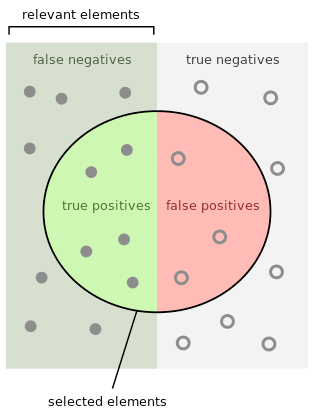
\includegraphics[scale=0.25]{figures/classifiers/evalterms.png}
\begin{equation*}
\textbf{Accuracy} = \frac{TP + TN}{Total} = \frac{200}{250} = 80\%
\end{equation*}
\end{frame}

\begin{frame}
\frametitle{Evaluation Metrics}
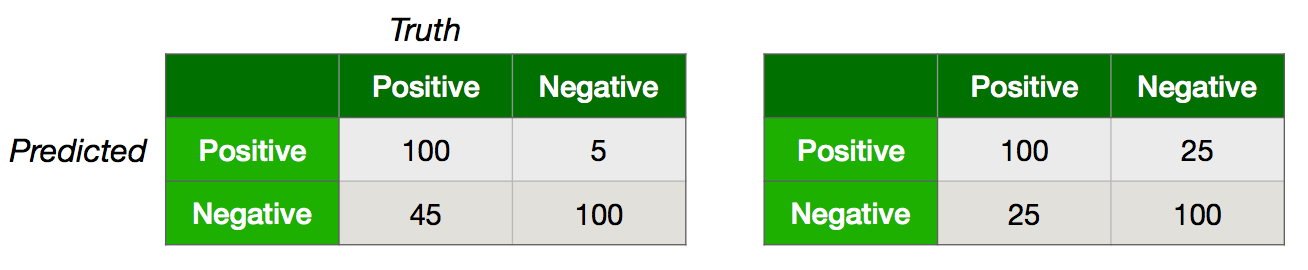
\includegraphics[scale=0.25]{figures/classifiers/evalex2.png}
\\
\centering
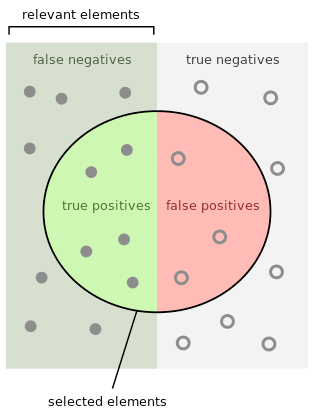
\includegraphics[scale=0.25]{figures/classifiers/evalterms.png}
\begin{equation*}
\textbf{Accuracy} = \frac{TP + TN}{Total} = \frac{200}{250} = 80\%
\end{equation*}
\end{frame}

\begin{frame}
\frametitle{Precision and Recall}
\centering
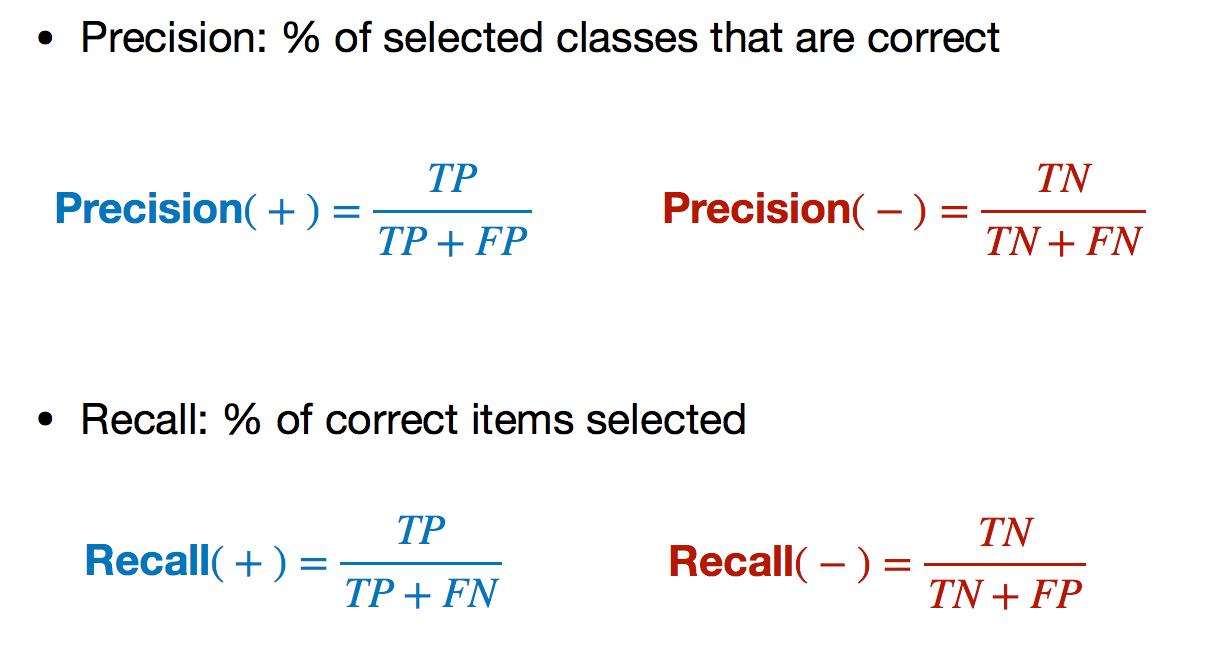
\includegraphics[scale=0.25]{figures/classifiers/prdef.png}
\end{frame}

\begin{frame}
\frametitle{Precision and Recall}
\centering
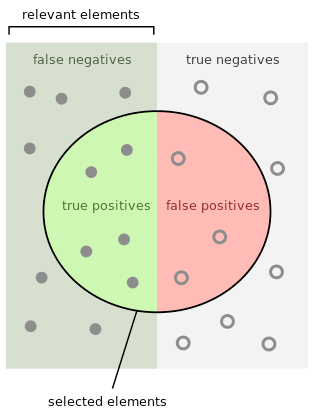
\includegraphics[scale=0.40]{figures/classifiers/evalterms.png}
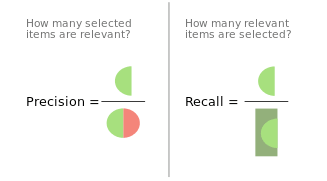
\includegraphics[scale=0.40]{figures/classifiers/pr.png}
\\
\footnotesize{from Wikipedia}
\end{frame}

\begin{frame}
\frametitle{F-Score}
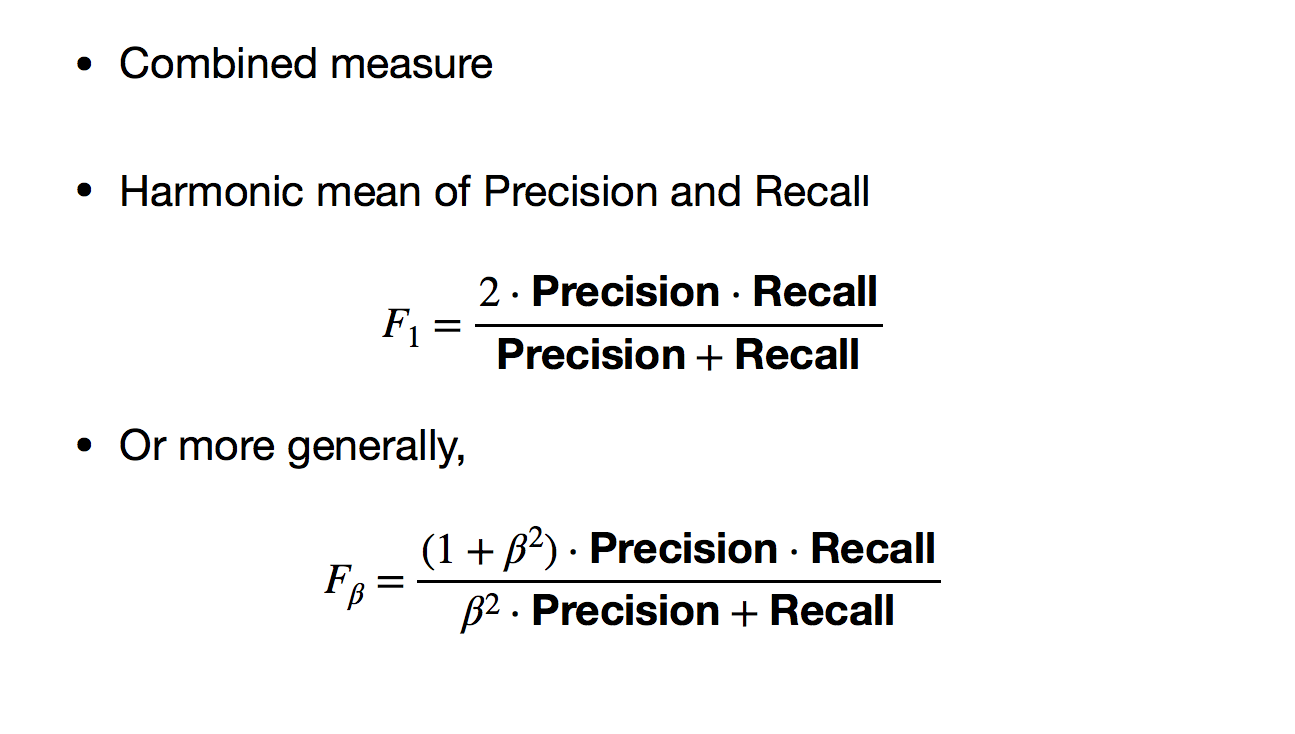
\includegraphics[scale=0.25]{figures/classifiers/fscore.png}
\end{frame}

\begin{frame}
\frametitle{Choosing Beta}
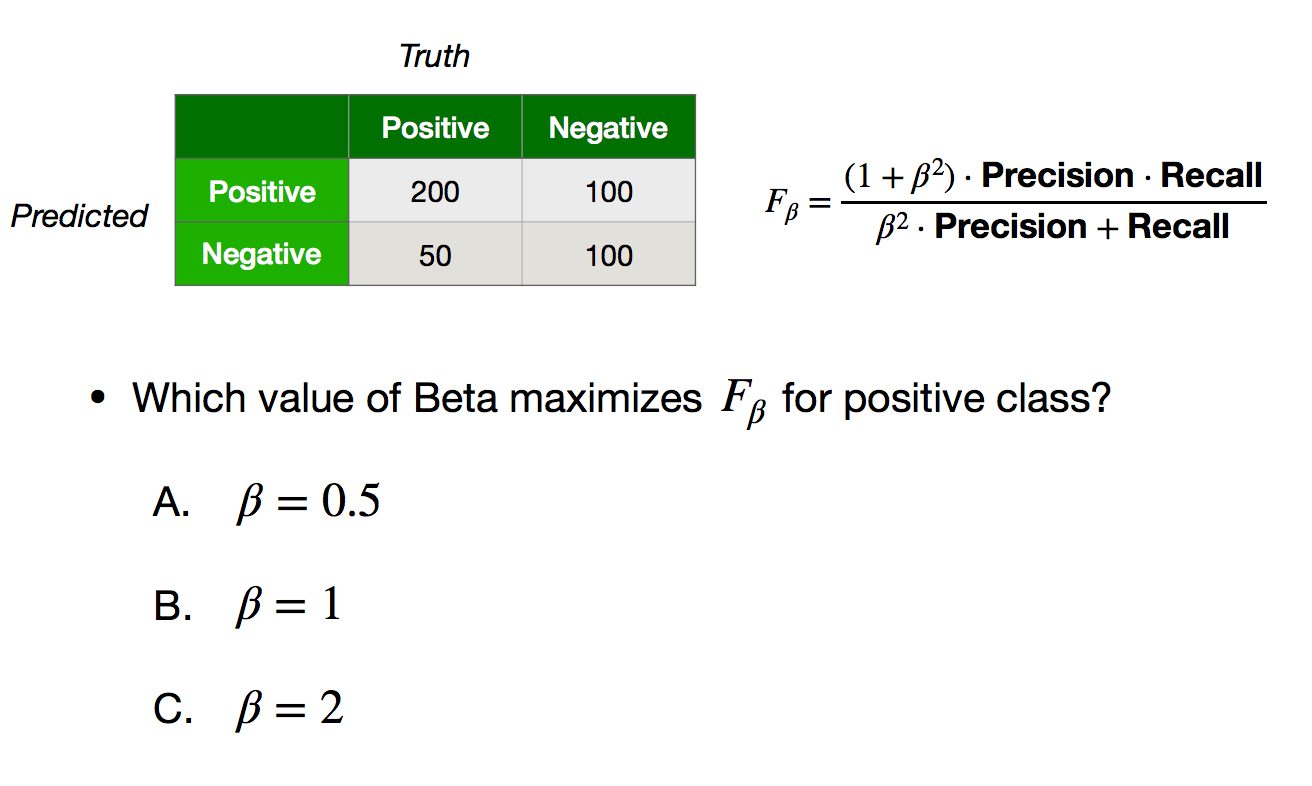
\includegraphics[scale=0.25]{figures/classifiers/beta.png}
\end{frame}

\begin{frame}
\frametitle{Aggregating scores}
\begin{itemize}[<+->]
\item We have Precision, Recall, F1 for each class
\item How to combine them for an overall score?
  \begin{itemize}
  \item Macro-average: Compute for each class, then average
  \item Micro-average: Collect predictions for all classes and jointly evaluate
  \end{itemize}
\end{itemize}
\end{frame}

\begin{frame}
\frametitle{Macro vs Micro average}
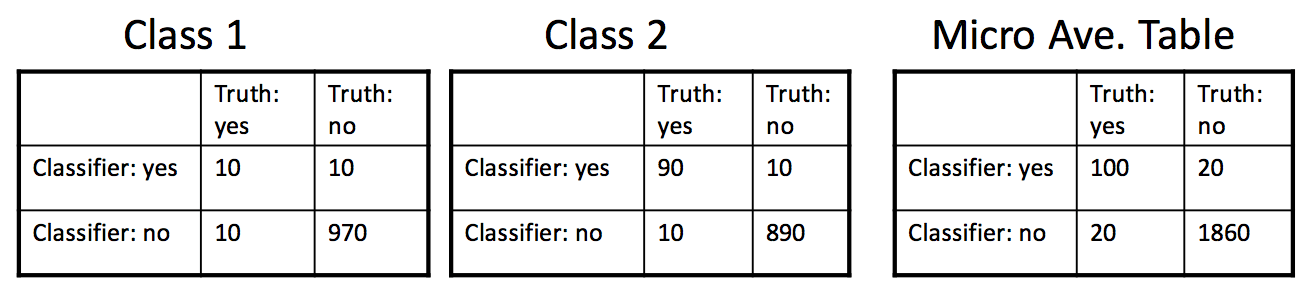
\includegraphics[scale=0.25]{figures/classifiers/averaging.png}
\begin{itemize}[<+->]
\item Macroaveraged precision: $(0.5+0.9)/2=0.7$
\item Microaveraged precision: $100/120=.83$
\item Microaveraged score is dominated by score on common classes
\end{itemize}
\end{frame}

\begin{frame}
\frametitle{Validation}

\includegraphics[scale=0.25]{figures/classifiers/splits.png}
\begin{itemize}[<+->]
\item Choose a metric: Precision/Recall/F1
\item Optimize for metric on {\color{green} Validation} (aka Development) set
\item Finally evaluate on ‘unseen’ {\color{red} Test} set
\item Cross-validation
  \begin{itemize}
  \item Repeatedly sample several train-val splits
  \item Reduces bias due to sampling errors \\
  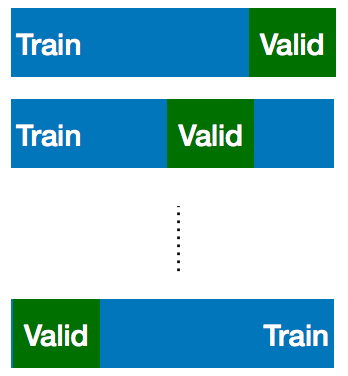
\includegraphics[scale=0.25]{figures/classifiers/cv.png}
  \end{itemize}
\end{itemize}
\end{frame}

\begin{frame}
\frametitle{Advantanges of Naive Bayes}
\begin{itemize}[<+->]
\item Very fast, low storage requirements
\item Robust to irrelevant features
\item Very good in domains with many equally important features
\item Optimal if the independence assumptions hold
\item Good dependable baseline for text classification
\end{itemize}
\end{frame}


\begin{frame}
\frametitle{When to use Naive Bayes}
\begin{itemize}[<+->]
\item Small data sizes: Naive Bayes is great! \note{high bias}.
 \\ Rule-based classifiers can work well too
\item Medium size datasets: More advanced classifiers might perform better (SVM, logistic regression)
\item Large datasets: Naive Bayes becomes competive again (most learned classifiers will work well)
\end{itemize}
\end{frame}

\begin{frame}
\frametitle{Failings of Naive Bayes (1)}
\begin{block}{Independence assumptions are too strong}
\begin{itemize}[<+->]
\item XOR problem: Naive Bayes cannot learn a decision boundary
\pause
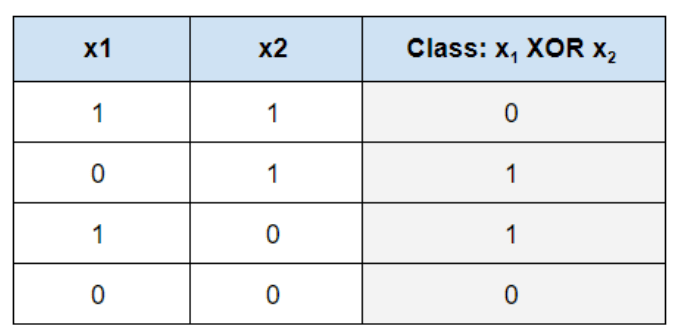
\includegraphics[scale=0.25]{figures/classifiers/xor.png}
\item Both variables are jointly required to predict class. Independence assumption broken!
\end{itemize}
\end{block}
\end{frame}

\begin{frame}
\frametitle{Failings of Naive Bayes (2)}
\begin{block}{Class Imbalance}
\begin{itemize}[<+->]
\item One or more classes have more instances than others
\item Data skew causes NB to prefer one class over the other
%\item Solution: Complement Naive Bayes \mycite{Rennie et al., 2003}
\end{itemize}
\end{block}
\end{frame}


\begin{frame}
\frametitle{Failings of Naive Bayes (3)}
\begin{block}{Weight magnitude errors}
\begin{itemize}[<+->]
\item Classes with larger weights are preferred
\item 10 documents with class=MA and “Boston” occurring once each
\item 10 documents with class=CA and “San Francisco” occurring once each
\item New document $d$: “Boston Boston Boston San Francisco San Francisco”
\pause
\\
\begin{equation*}
P(\text{class}=\text{CA} | d) > P(\text{class} = \text{MA} | d)
\end{equation*}
\end{itemize}
\end{block}
\end{frame}

\begin{frame}
\frametitle{Naive Bayes Summary}
\begin{itemize}[<+->]
\item Domain knowledge is crucial to selecting good features
\item Handle class imbalance by re-weighting classes
\item Use log scale operations instead of multiplying probabilities
\begin{equation*}
P(c_{NB}) = \argmax_{c_j \in C} \log P(c_j) + \sum_{i} \log P(x_i | c_j)
\end{equation*}
\item Model is now just max of sum of weights
\end{itemize}
\end{frame}


\author{Angel Xuan Chang \\ 
  {\color{RoyalBlue!70}{\href{http://angelxuanchang.github.io/nlp-class}{angelxuanchang.github.io/nlp-class}}} \\
  {\color{gray}{adapted from lecture slides from Anoop Sarkar}}
}

\section{Log linear models}
\frame{\tableofcontents[currentsection]}

\begin{frame}
\frametitle{Log linear model}
\begin{itemize}[<+->]
\item The model classifies input into output labels $y \in {\cal Y}$
\item Let there be $m$ features, $f_k(\textbf{x}, y)$ for $k = 1, \ldots, m$
\item Define a parameter vector $\textbf{v} \in \mathbb{R}^m$
\item Each $(\textbf{x}, y)$ pair is mapped to score:
\[ s(\textbf{x}, y) = \sum_k v_k \cdot f_k(\textbf{x}, y) \]
\item Using inner product notation:
\begin{eqnarray*}
\textbf{v} \cdot \textbf{f}(\textbf{x}, y) & = & \sum_k v_k \cdot f_k(\textbf{x}, y) \\
s(\textbf{x}, y) & = & \textbf{v} \cdot \textbf{f}(\textbf{x}, y) 
\end{eqnarray*}
\item To get a probability from the score: Renormalize! 
\[ \Pr(y \mid \textbf{x}; \textbf{v}) = \frac{exp\left(s(\textbf{x}, y)\right)}{\sum_{y' \in {\cal Y}} exp\left(s(\textbf{x}, y')\right)} \]
\end{itemize}
\end{frame}

\begin{frame}
\frametitle{Log linear model}
\begin{itemize}[<+->]
\item The name `log-linear model' comes from:
\[ \log \Pr(y \mid \textbf{x}; \textbf{v}) = \underbrace{\textbf{v} \cdot \textbf{f}(\textbf{x}, y)}_{\textrm{linear term}} - \underbrace{\log \sum_{y'} exp\left( \textbf{v} \cdot \textbf{f}(\textbf{x}, y') \right)}_{\textrm{normalization term}} \]
\item Once the weights $\textbf{v}$ are learned, we can perform predictions using these features.
\item The goal: to find $\textbf{v}$ that maximizes the log likelihood $L(\textbf{v})$ of the labeled training set containing $(\textbf{x}_i, y_i)$ for $i = 1 \ldots n$
\begin{eqnarray*}
L(\textbf{v}) &=& \sum_{i} \log \Pr(y_i \mid \textbf{x}_i; \textbf{v}) \\
&=& \sum_i \textbf{v} \cdot \textbf{f}(\textbf{x}_i, y_i) - \sum_i \log \sum_{y'} exp\left( \textbf{v} \cdot \textbf{f}(\textbf{x}_i, y') \right) 
\end{eqnarray*}
\end{itemize}
\end{frame}

\begin{frame}
\frametitle{Log linear model}
\begin{itemize}[<+->]
\item Maximize:
\begin{eqnarray*}
L(\textbf{v}) &=& \sum_i \textbf{v} \cdot \textbf{f}(\textbf{x}_i, y_i) - \sum_i \log \sum_{y'} exp\left( \textbf{v} \cdot \textbf{f}(\textbf{x}_i, y') \right) 
\end{eqnarray*}
\item Calculate gradient:
\begin{eqnarray*}
\lefteqn{\left. \frac{d L(\textbf{v})}{d \textbf{v}} \right|_{\textbf{v}} } \\
&=& \sum_i \textbf{f}(\textbf{x}_i, y_i) - \sum_i \frac{1}{\sum_{y''} exp\left(\textbf{v} \cdot \textbf{f}(x_i, y'')\right)} \\
&& \sum_{y'} \textbf{f}(\textbf{x}_i, y')  \cdot exp\left( \textbf{v} \cdot \textbf{f}(\textbf{x}_i, y') \right) \pause \\
&=& \sum_i \textbf{f}(\textbf{x}_i, y_i) - \sum_i \sum_{y'} \textbf{f}(\textbf{x}_i, y') \frac{exp\left( \textbf{v} \cdot \textbf{f}(\textbf{x}_i, y') \right)}{\sum_{y''} exp\left(\textbf{v} \cdot \textbf{f}(x_i, y'')\right)} \\
&=& \underbrace{\sum_i \textbf{f}(\textbf{x}_i, y_i)}_{\textrm{Observed counts}} - \underbrace{\sum_i \sum_{y'} \textbf{f}(\textbf{x}_i, y') \Pr(y' \mid \textbf{x}_i; \textbf{v})}_{\textrm{Expected counts}}
\end{eqnarray*}
\end{itemize}
\end{frame}

\begin{frame}
\frametitle{Gradient ascent}
\begin{itemize}[<+->]
\item Init: $\textbf{v}^{(0)} = \textbf{0}$
\item $t \leftarrow 0$
\item Iterate until convergence:
\begin{itemize}[<+->]
\item Calculate: $\Delta = \left. \frac{d L(\textbf{v})}{d \textbf{v}}  \right|_{\textbf{v} = \textbf{v}^{(t)}}$
\item Find $\beta^\ast = \arg\max_\beta L(\textbf{v}^{(t)} + \beta \Delta)$
\item Set $\textbf{v}^{(t+1)} \leftarrow \textbf{v}^{(t)} + \beta^\ast \Delta$
\end{itemize}
\end{itemize}
\end{frame}

\begin{frame}
\frametitle{Learning the weights: $\textbf{v}$: Generalized Iterative
  Scaling}
\begin{tabbing}
$f^\# = max_{x,y} \sum_{j} f_j(x, y)$ \\
(the maximum possible feature value; needed for scaling) \pause \\
Initialize $\textbf{v}^{(0)}$ \pause \\
For \= each iteration $t$ \\
\> \texttt{expected[j]} $\leftarrow$ 0 for j = 1 .. \# of features \pause \\
\> For \= i = 1 to $\mid \textrm{training data} \mid$ \\
\>     \> For \= each feature $f_j$ \\
\>     \>     \> \texttt{expected[j]} += $f_j(x_i, y_i) \cdot P(y_i \mid x_i; \textbf{v}^{(t)})$ \pause \\
\> For \= each feature $f_j(x,y)$ \\
\>     \> \texttt{observed[j]} = $f_j(x, y) \cdot \frac{c(x,y)}{\mid \textrm{training data} \mid}$ \pause \\ 
\> For \= each feature $f_j(x,y)$ \\
\>     \> $v_j^{(t+1)} \leftarrow v_j^{(t)} \cdot \sqrt[f^\#]{\frac{\texttt{observed[j]}}{\texttt{expected[j]}}}$ 
\end{tabbing}
\par\noindent
\small{cf. Goodman, NIPS '01}
\end{frame} 


\section*{Acknowledgements}

\begin{frame}
\centering
\begin{alertblock}{Acknowledgements}
Many slides borrowed or inspired from lecture notes by Michael Collins, Chris Dyer, Kevin Knight, Philipp Koehn, Adam Lopez, Graham Neubig and Luke Zettlemoyer from their NLP course materials. 

\bigskip

All mistakes are my own.

\bigskip

A big thank you to all the students who read through these notes and helped me improve them.

\end{alertblock}
\end{frame}



\end{document}

\begin{frame}
\frametitle{Maximum Entropy}
\begin{itemize}[<+->]
\item The log-linear model has an interpretation as a {\it maximum entropy} model.
\item For observed events, maximize likelihood. For unobserved events, from all
consistent models pick the one with maximum entropy.
\item The maximum entropy principle: related to Occam's razor and
  other similar justifications for scientific inquiry
\item Make the minimum possible assumptions about unseen data
\item Also: Laplace's {\em Principle of Insufficient Reason}: when one
  has no information to distinguish between the probability of two
  events, the best strategy is to consider them equally likely
\end{itemize}
\end{frame}

\begin{frame}
\frametitle{Logistic Regression}
\begin{itemize}
\item models effects of explanatory variables on binary valued
  variable
\item observations ${\bf x} = \{x_1, \ldots, x_j\}$ with success given
  by $q({\bf x})$: \[ q({\bf x}) = \frac{e^{g({\bf x})}}{1 + e^{g({\bf
  x})}} \] and \[ g({\bf x}) = \beta_0 + \sum_{j=1}^{k} \beta_j x_j \]
\end{itemize} 
\end{frame} 

\begin{frame}
\frametitle{Logistic Regression}
\begin{itemize}
\item probability that observations lead to success, or $p(a=1 \mid
  b)$:
 \[ p(a=1 \mid b) = \frac{e^{g(b)}}{1 + e^{g(b)}} \] where
 \[ g(b) = \beta_0 f_0(1,b) + \sum_{j=1}^{k} \beta_j f_j(1,b) \]
\item $\beta_j = \textrm{log} \alpha_j$, $f_0(1,b) = 1$ and $f_j(1,b) = x_j$
\end{itemize} 
\end{frame} 
